\begin{figure}[tp]
  \usetikzlibrary{shapes.arrows}
  \definecolor{LightColor}{rgb}{1.0,0.901,0.805}
  \definecolor{EmptyColor}{HTML}{DCE2E6};

  \definecolor{tile0}{HTML}{DABDE4}
  \definecolor{tile1}{HTML}{B8DBF4}
  \definecolor{tile2}{HTML}{B5EDCD}
  \definecolor{tile3}{HTML}{FBEBA7}
  \definecolor{tile4}{HTML}{F9C1BB}
  \definecolor{tile5}{rgb}{1, 1, 1}

  \tikzstyle{array_element}=[rectangle,
                             minimum height=1.0cm, 
                             minimum width=1.0cm, 
                             minimum size=1.0cm,
                             draw=black,
                             rounded corners=2.5, ]

\begin{adjustbox}{minipage=\textwidth, scale=0.9}
  \centering
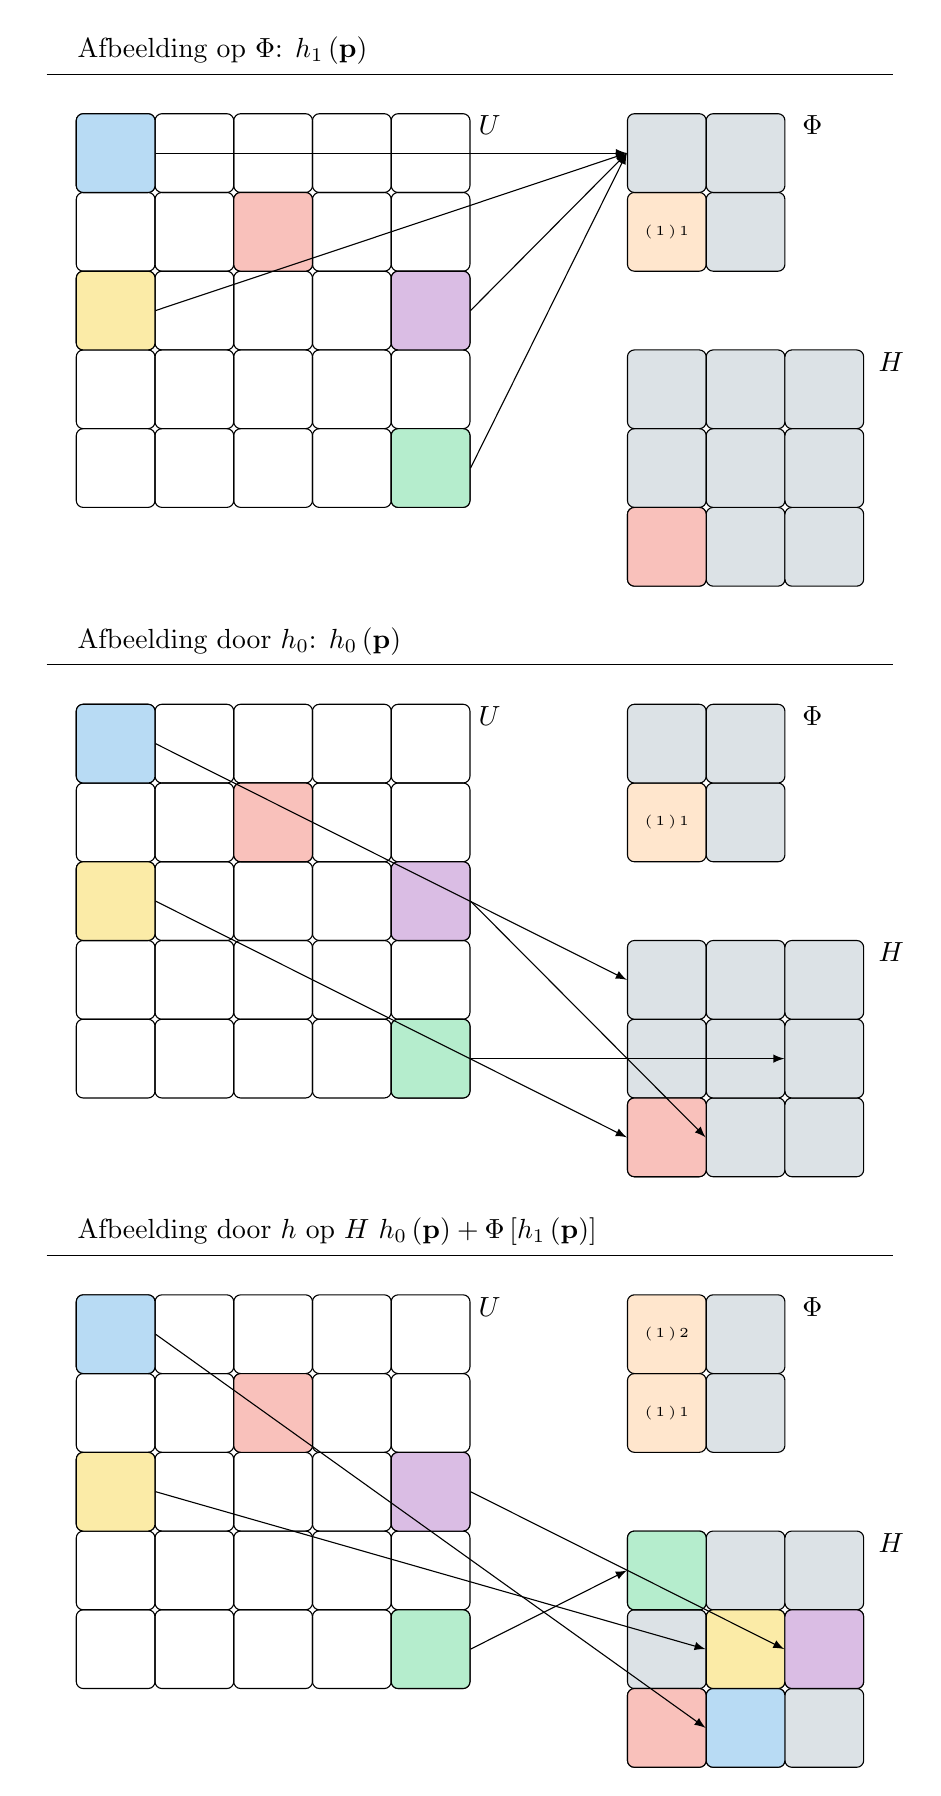
\begin{tikzpicture}
    % ---------------------------------------------------------------------------------------------------------
    %  Start situatie
    \node at (-1cm, 5cm) (line-1-l) {};
    \node at (10cm, 5cm) (line-1-r) {};
    \draw[-] (line-1-l) -- (line-1-r) node[pos=0.025, above right] {Afbeelding op $\Phi$: $h_1\left( \mathbf{p} \right)$};
    
    \node at (7cm, 3cm) (PhiC0) [array_element, fill=LightColor] {\tiny $\begin{pmatrix}1 \\ 1\end{pmatrix}$};
    \node at (8cm, 3cm) (PhiC1) [array_element, fill=EmptyColor] {};
    \node at (7cm, 4.0cm) (PhiC2) [array_element, fill=EmptyColor] {};
    \node at (8.0cm, 4.0cm) (PhiC3) [array_element, fill=EmptyColor] {};    
    
    \foreach \la in {0,...,2} {
        \foreach \lb in {0,...,2} {
            \node at (1.0cm * \la + 7cm, 1.0cm * \lb - 1.0cm) (H\la\lb) [array_element, fill=EmptyColor] {};
        }
    }
    \node at (7cm, -1.0cm) (HC1) [array_element, fill=tile4] {};

    \foreach \la in {0,...,4} {
        \foreach \lb in {0,...,4} {
            \node at (1.0cm * \la, 1.0cm * \lb) () [array_element] {};
        }
    }
    
    \node at (0.0cm, 4.0cm) (UC0) [array_element, fill=tile1] {};
    \node at (0.0cm, 2.0cm) (UC1) [array_element, fill=tile3] {};
    \node at (4.0cm, 2.0cm) (UC2) [array_element, fill=tile0] {};
    \node at (4.0cm, 0.0cm) (UC3) [array_element, fill=tile2] {};
    \node at (2.0cm, 3.0cm) (UC4) [array_element, fill=tile4] {};

    \node at(4.75cm, 4.35cm) (U) [] {$U$};
    \node at(4.75cm, 4.35cm - 7.5cm) (U) [] {$U$};
    \node at(4.75cm, 4.35cm - 15cm) (U) [] {$U$};
    
    \node at(8.85cm, 4.35cm) (U) [] {$\Phi$};
    \node at(8.85cm, 4.35cm - 7.5cm) (U) [] {$\Phi$};
    \node at(8.85cm, 4.35cm - 15cm) (U) [] {$\Phi$};
    
    \node at(9.85cm, 1.35cm) (U) [] {$H$};
    \node at(9.85cm, 1.35cm - 7.5cm) (U) [] {$H$};
    \node at(9.85cm, 1.35cm - 15cm) (U) [] {$H$};
    
    \draw[-latex] (UC1.east) -- (PhiC2.west);
    \draw[-latex] (UC2.east) -- (PhiC2.west);
    \draw[-latex] (UC3.east) -- (PhiC2.west);
    \draw[-latex] (UC0.east) -- (PhiC2.west);

   % ---------------------------------------------------------------------------------------------------------
    \node at (-1cm, -2.5cm) (line-2-l) {};
    \node at (10cm, -2.5cm) (line-2-r) {};
    \draw[-] (line-2-l) -- (line-2-r) node[pos=0.025, above right] {Afbeelding door $h_0$: $h_0\left( \mathbf{p} \right)$};

    \node at (7cm, 3cm -7.5cm) (PhiC0) [array_element, fill=LightColor] {\tiny $\begin{pmatrix}1 \\ 1\end{pmatrix}$};
    \node at (8cm, 3cm -7.5cm) (PhiC1) [array_element, fill=EmptyColor] {};
    \node at (7cm, 4.0cm -7.5cm) (PhiC2) [array_element, fill=EmptyColor] {};
    \node at (8.0cm, 4.0cm  -7.5cm) (PhiC3) [array_element, fill=EmptyColor] {};    
    
    \foreach \la in {0,...,2} {
        \foreach \lb in {0,...,2} {
            \node at (1.0cm * \la + 7cm, 1.0cm * \lb - 1.0cm - 7.5cm) (H\la\lb) [array_element, fill=EmptyColor] {};
        }
    }
    \node at (7cm, -1.0cm - 7.5cm) (HC1) [array_element, fill=tile4] {};

    \foreach \la in {0,...,4} {
        \foreach \lb in {0,...,4} {
            \node at (1.0cm * \la, 1.0cm * \lb - 7.5cm) () [array_element] {};
        }
    }

    \node at (0.0cm, 4.0cm - 7.5cm) (UC0) [array_element, fill=tile1] {};
    \node at (0.0cm, 2.0cm - 7.5cm) (UC1) [array_element, fill=tile3] {};
    \node at (4.0cm, 2.0cm - 7.5cm) (UC2) [array_element, fill=tile0] {};
    \node at (4.0cm, 0.0cm - 7.5cm) (UC3) [array_element, fill=tile2] {};
    \node at (2.0cm, 3.0cm - 7.5cm) (UC4) [array_element, fill=tile4] {};
    
    \draw[-latex] (UC1.east) -- (H00.west) ;%node[pos=0.08, above right] {$h_0$};
    \draw[-latex] (UC2.east) -- (H10.west);% node[pos=0.08, below] {$h_0$};
    \draw[-latex] (UC3.east) -- (H21.west);% node[pos=0.08, above right] {$h_0$};
    \draw[-latex] (UC0.east) -- (H02.west);% node[pos=0.08, above] {$h_0$};

   % ---------------------------------------------------------------------------------------------------------
    \node at (-1cm, 5cm - 15cm) (line-3-l) {};
    \node at (10cm, 5cm - 15cm) (line-3-r) {};
    \draw[-] (line-3-l) -- (line-3-r) node[pos=0.025, above right] {Afbeelding door $h$ op $H$ $h_0\left( \mathbf{p} \right) + \Phi\left[ h_1 \left( \mathbf{p} \right) \right]$};

    \node at (7cm, 3cm -15cm) (PhiC0) [array_element, fill=LightColor] {\tiny $\begin{pmatrix}1 \\ 1\end{pmatrix}$};
    \node at (8cm, 3cm -15cm) (PhiC1) [array_element, fill=EmptyColor] {};
    \node at (7cm, 4.0cm -15cm) (PhiC2) [array_element, fill=LightColor] {\tiny $\begin{pmatrix}1 \\ 2\end{pmatrix}$};
    \node at (8.0cm, 4.0cm  -15cm) (PhiC3) [array_element, fill=EmptyColor] {};    
    
    \foreach \la in {0,...,2} {
        \foreach \lb in {0,...,2} {
            \node at (1.0cm * \la + 7cm, 1.0cm * \lb - 1.0cm - 15cm) (H\la\lb) [array_element, fill=EmptyColor] {};
        }
    }
    \node at (7cm, -16cm) (HC1) [array_element, fill=tile4] {};
    \node at (8cm, -16cm) (HC2) [array_element, fill=tile1] {};
    \node at (7cm, -14cm) (HC3) [array_element, fill=tile2] {};
    \node at (8cm, -15cm) (HC4) [array_element, fill=tile3] {};
    \node at (9cm, -15.0cm) (HC5) [array_element, fill=tile0] {};

    \foreach \la in {0,...,4} {
        \foreach \lb in {0,...,4} {
            \node at (1.0cm * \la, 1.0cm * \lb - 15cm) () [array_element] {};
        }
    }
    
    \node at (0.0cm, 4.0cm-15cm) (UC0) [array_element, fill=tile1] {};
    \node at (0.0cm, 2.0cm-15cm) (UC1) [array_element, fill=tile3] {};
    \node at (4.0cm, 2.0cm-15cm) (UC2) [array_element, fill=tile0] {};
    \node at (4.0cm, 0.0cm-15cm) (UC3) [array_element, fill=tile2] {};
    \node at (2.0cm, 3.0cm-15cm) (UC4) [array_element, fill=tile4] {};
    
    \draw[-latex] (UC1.east) -- (HC4.west);
    \draw[-latex] (UC2.east) -- (HC5.west);
    \draw[-latex] (UC3.east) -- (HC3.west);
    \draw[-latex] (UC0.east) -- (HC2.west);
\end{tikzpicture}
\end{adjustbox}
  \caption{De toekenning van een enkele offset-waarde om de perfecte spatiale hashfunctie $\mathit{h}\left(\mathbf{p}\right)$ op te bouwen.}
  \label{fig:hs-spatiale-hashfunctie-update}
\end{figure}
